
%%%%%%%%%% Conference Latex Template for the university center of Tipaza - Algeria
%%%%%%%%%% created by F.CHABNI




\documentclass{report}
\usepackage{ctex}
\usepackage{geometry}
\usepackage{graphicx}
\usepackage{amsmath}
\usepackage{cite}
\usepackage{subcaption}
\usepackage{booktabs}
\usepackage{multirow}
% \usepackage{graphicx}
\usepackage[table,xcdraw]{xcolor}
\title{自主移动车文献综述和原型设计}
\author{邱璟祎, 周俊豪, 张峻瑜\\
  (按姓名首字母排序)
}
\geometry{a4paper,scale=0.8}
\begin{document}
\maketitle
\tableofcontents
\newpage
\chapter{引言}

在当今这个技术飞速发展的时代,自动化和智能化已成为工业生产和日常生活的关键趋势。在自动化物流系统中,智能小车扮演着核心角色,其发展和应用吸引了广泛的关注。本研究旨在响应这一时代的需求,设计并开发一款AGV智能小车。本文将从课程任务出发,对各个任务模块进行细致分析和分解,通过文献综述梳理现有解决方案,并提出一个初步的设计方案。

本文所探讨的智能小车是一种能够在自动导引车(AGV)系统中自主完成移动、货物抓取、运输和卸载的自动化设备。在对智能小车的需求进行深入分析和任务分解后,本文将从机械设计、路径追踪算法和避障策略三个关键技术领域进行详尽的文献调研,并进行综合性评述。我们将总结这些领域的现有技术,并评估它们在智能小车设计中的潜力和局限性。

在广泛调研的基础上,本文将结合需求分析和文献综述的结果,提出一套创新的设计方案。该方案将涵盖智能小车的机械结构、测量技术、路径追踪与避障算法、数据传输和驱动系统等关键技术要素。同时,本文也将探讨该方案的实施可行性及其可能面临的技术挑战。

通过本研究,我们期望为智能小车的设计提供有价值的参考和指导,为智能小车市场的设计提供新的思路,促进自动化物流技术的发展,并为工业自动化和智能运输系统的创新贡献力量。



\chapter{需求分析}
课程任务为:设计并实现一个机电系统,按照规定路线,在2种不同场地,将指定物品从一个指定位置运输到另一指定位置。两种场地分别需要实现循迹和避障的功能。为了完成这个任务,将任务分解为机械结构、电气、测量、算法和系统软件五个方面的内容。
\section{机械结构}
\label{sec:label}
\subsection{车体结构}
\label{subsec:label}
\begin{enumerate}
\item 整体尺寸:避障部分场地的障碍物间距不小于350mm,故小车的整体尺寸应当小于该距离。
\item 驱动与转弯方式:驱动方式可以选择轮式或者履带式,转弯方式可以采用差速转向或者麦克纳姆轮转向。
  \item 车体空间结构:车上需要装载驱动电机、控制板、传感器等元件以及电子线路,可以考虑设计多层结构,同时需要考虑重心的稳定性和小车的承重性能。
\end{enumerate}
\subsection{抓取机构}
\label{subsec:label}
\begin{enumerate}
\item 机械爪及舵机:货物尺寸为直径30mm,高40mm,其重量为50g,因此抓取结构中的机械爪需与货物尺寸相匹配,且相应舵机需要有足够的力矩。
  \item 抓取结构大小与工作空间:因小车本身体积有限,因此抓取结构不应过大。除此之外,还需考虑抓取结构的工作空间,如不能遮挡摄像头视野等。
  \end{enumerate}
  \newpage
\section{电气}
\label{subsec:label}
\subsection{控制器硬件}
\label{subsec:label}
常用的包括编程调试方便,主要串行执行的CPU和并发速度快,可靠性好,调试困难的FPGA,可以根据功能需求、计算能力等方面的约束进行选取。
\subsection{电机与驱动}
\label{subsec:label}
常用的驱动电机包括航模电机和直流电机等,需要根据驱动力要求、电路负载要求等进行选取。
\subsection{电源}
\label{subsec:label}
单片机、电机、舵机等不同元器件的所需电压不同,需要进行相应的电源与二次电源的选择,具体选择将在原理方案设计部分确定。
\subsection{通讯}
\label{subsec:label}
需要实现的数据通讯任务包括实时图像、指令数据、状态参数和舵机命令等,可以采用USB数据线的有线通讯方式或者蓝牙等无线通讯方式,具体选择需要根据传输数据量、数据传输延时和硬件接口等因素确定。
\section{测量}
\label{sec:label}
需要传感器传回的信息主要包括图像灰度、距离、小车自身的位置和姿态等等,可能需要红外传感器、超声传感器、线阵CCD传感器、里程计和陀螺仪等,需要根据需求进行选取,同时要和车体结构相匹配。
\section{算法}
\label{sec:label}
循迹和避障的算法现有的文献和其他资料都有很多内容,将在后面文献综述部分加以阐述,并在设计部分进行选择。

\section{系统软件}
\label{sec:label}
系统软件需要根据功能和算法进行划分,并且和实际硬件进行对应,从而实现各个模块之间的交互。


\chapter{自主移动车文献综述}
\label{sec:label}


\section{机械设计研究综述}
\subsection{运动方式}
\label{subsec:label}
目前自主移动车的运动方式主要分为轮式和履带式,下面将分别论述这两种方式的特点。
\subsubsection{轮式运动}
\label{subsec:label}
轮式运动是自主移动车辆(Autonomous Mobile Vehicles, AMVs)中普遍采用的一种驱动方式,其核心功能是通过一个或多个轮子实现车辆的移动。这种设计可以采用标准的轮胎或灵活的全方位轮(Omni-Directional Wheels, ODWs),特别适合在平坦且结构简单的环境条件下使用。轮式驱动的优势在于其高度的机动性、简化的结构设计、强大的操控性能以及卓越的安全特性。

根据驱动机制的不同,轮式运动车辆可以被进一步分类为单驱动轮、双驱动轮和多驱动轮三种类型。单驱动轮系统通常应用于三轮的自动引导车(AGV),而双驱动轮系统则多见于四轮AGV。这两种驱动方式的共同之处在于,仅部分车轮配备驱动力,从而减少所需的驱动电机数量,降低车辆的总重量,并节省宝贵的内部空间。然而,这种设计有时可能导致由于重量分布不均,非驱动轮一侧的附着力不足,进而影响车辆的转向性能。

与此相对,多驱动轮AGV的每个轮子都与驱动电机相连,这提供了更强的驱动力和更均匀的重量分布。尽管如此,这种设计在提升驱动性能的同时,可能会在一定程度上降低车辆的灵活性。

\subsubsection{履带式运动}
\label{subsec:label}
采用履带驱动的自动引导车(AGV)因其独特的设计,在复杂地形如雪地和斜坡上展现出卓越的附着力和稳定性。这些AGV的地面压力较低,摩擦系数较高,使其能够承载较重的载荷。然而,与轮式AGV相比,履带式AGV的制造成本较高,且运行速度相对较慢。

履带式AGV的设计允许它们在承受重载的同时,在不平坦或恶劣的地面条件下保持稳定。它们的履带结构提供了较大的接触面积,这不仅减少了对地面的压力,还增加了与地面的摩擦力,从而提高了车辆的牵引力。虽然在成本和速度方面,履带式AGV可能不如轮式AGV,但它们在特定应用场景下的优势是无可替代的。

\newpage
\subsection{转向方式}
\label{subsec:label}
目前已有的AGV中,转向方式大部分都可以归结为差速转向和麦克纳姆轮转向两大类,下面将分别进行叙述
\subsubsection{差速转向\cite{chasu}}
\label{subsec:label}
在车辆设计中,采用四轮驱动系统并结合阿克曼转向几何学原理,可以显著提高车辆在转向时的稳定性和操控性。当车辆的前轮和后轮均具备驱动能力时,根据阿克曼原理,车辆在转向过程中,四个轮胎似乎围绕一个共同的中心点旋转,这种设计有助于保持车辆行驶的稳定性。

将车辆的几何中心视为质心,并在理想条件下忽略诸如路面条件变化等外部因素,我们可以构建一个四轮驱动且具有差速转向功能的小车的运动学模型。这一模型不仅能够描述车辆在直线行驶和转向时的运动特性,还能够为车辆控制系统的设计提供理论基础。

运动学模型的建立通常涉及对车辆动力学的简化和抽象,通过数学表达式来描述车辆的运动状态。在示意图中,我们可以清晰地看到车辆的转向机制和各轮子的相对位置,这有助于我们更好地理解车辆在不同转向条件下的运动规律。

\begin{figure}[ht]
  \centering
  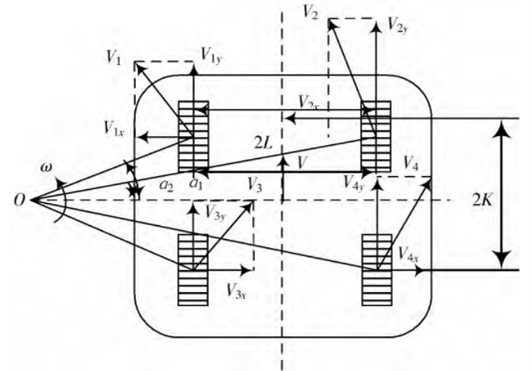
\includegraphics[width=0.5\textwidth]{figures/chasu.png}
  \caption{差速转向受力分析}
\end{figure}
\newpage
$\alpha_1$和$\alpha_2$分别为前左轮和后左轮,前右轮和右轮的转角;2L 为左右轮距离; 2K 为前后轮轴距;$v$和$\omega$分别为车子质心的线速度和角速度,$V_1,V_2,V_3,V_4$分别为各个轮中心的实际运动方向。由图 可以得出各速度和转角的关系:
\[\begin{gathered}
V_{1}=\omega R_{1}=\omega\frac{K}{sin\alpha_{1}}\\
V_{2}=\omega R_{2}=\omega\frac{K}{sin\alpha_{2}} \\
V_{3}=V_{1}=\omega\frac{K}{sin\alpha_{1}} \\
V_{4}=V_{2}=\omega\frac{K}{sin\alpha_{2}}\\
V_{1y}=V_{1}cos\alpha_{1}= \omega\frac{K}{tan\alpha_{1}}=\omega(R-L)\\
V_{2y}=V_{2}cos\alpha_{2}= \omega\frac{K}{tan\alpha_{2}}=\omega(R+L)\\
V_{3y}=V_{3}cos\alpha_{1}= \omega\frac{K}{tan\alpha_{1}}=\omega(R-L)\\
V_{4y}=V_{4}cos\alpha_{2}= \omega\frac{K}{tan\alpha_{2}}=\omega(R+L)
\end{gathered}\]
式中$R=\frac v\omega $。

则电机的角速度为:$\omega_n=\frac{V_{ny}i}r,n=1,2,3,4$

式中$i$为减速器的减速比,$r$为车轮半径。


\subsubsection{麦克纳姆轮转向\cite{mac}}
\label{subsec:label}
麦克纳姆驱动系统赋予移动平台在二维平面内沿三个独立方向移动的能力。这一系统通过四个独立控制的轮子实现,每个轮子以不同的速度旋转,协同工作以提供全向移动的能力。每个轮子对整体移动方向和速度的贡献都是至关重要的。

与传统轮子不同,麦克纳姆轮的特点是其圆周上均匀分布着多个小型辊子,这些辊子的轴线与轮子中心轴线形成特定角度,如45度。这些辊子的轮廓线与轮子的基本圆形轮廓相匹配,确保了它们始终与地面保持接触。这些辊子能够自由旋转,使得轮子主要承受垂直于地面的力,而地面对辊子的摩擦力则转化为滚动摩擦,其影响可以忽略不计。

由于这种设计,轮子与地面的接触不是沿着轮子的圆周,而是以一定角度作用。这允许轮子在受到驱动力的同时,在另一个方向上实现自由移动。通过这四个轮子的协同作用,可以产生多种不同的受力情况,从而使平台能够在二维空间内沿三个方向自由移动。


用$R$表示全向轮轴心到轮外廓圆周面的距离即轮的半径;$V_i$表示第$i$轮的速度;$\alpha$表示辊子轴线与全向轮轴线夹角;$\omega_i$表示全向轮绕轮轴的转速;i=1,2,3,4,分别代表左前轮、右前轮、左后轮、右后轮。联立可得矩阵方程:
\[ V_i=\begin{pmatrix}R\\4\end{pmatrix}\begin{bmatrix}1&1&1&1\\\tan\alpha&-\tan\alpha&-\tan\alpha&\tan\alpha\\-\frac{1}{l_0}&\frac{1}{l_0}&-\frac{1}{l_0}&\frac{1}{l_0}\end{bmatrix}\begin{bmatrix}\omega_1\\\omega_2\\\omega_3\\\omega_4\end{bmatrix}\]

式中$l_0=$W+ Lcos$\alpha$,其中 W 为移动平台宽度,L 为其前后轮轴距;而$\alpha$取
$45^{\circ}$,其正负号已被提出,不再区分正负。逆运动学方程为:
\[\begin{bmatrix}\omega_1\\\omega_2\\\omega_3\\\omega_4\end{bmatrix}=\text{K}\begin{bmatrix}V_y\\V_x\\\omega\end{bmatrix}=\begin{pmatrix}\frac{1}{R}\end{pmatrix}\begin{bmatrix}1&cot\alpha&-l_0\\1&-cot\alpha&l_0\\1&-cot\alpha&-l_0\\1&cot\alpha&l_0\end{bmatrix}\begin{bmatrix}V_y\\V_x\\\omega\end{bmatrix}\]
总的来说,麦克纳姆轮转向具有高效率、高灵活性的特点。
\begin{figure}[ht]
  \centering
  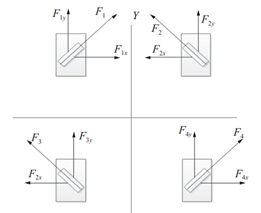
\includegraphics[width=0.5\textwidth]{figures/mac.png}
  \caption{麦克纳姆轮受力分析 }
\end{figure}
\subsection{抓取机构}
\label{subsec:label}
机械臂末端的抓取机构可以采用机械手爪、吸盘和仿生结构三种形式,它们具体的特点如下:
\subsubsection{机械手爪}
\label{subsec:label}
机械手爪的分类基于其驱动原理,可分为五大类:气动型、电动型、液压型、电磁型和热能型。气动型机械手爪利用压缩空气实现其抓取动作,其优点在于成本效益高和响应速度快,但需持续供应压缩空气,且在控制精度上存在局限。电动型机械手爪以电动机为动力源,通过齿轮、皮带或丝杠等机械传动元件传递动力,具有高精度控制和均衡的力矩输出,但可能因结构复杂性而增加成本。液压型机械手爪通过液压系统提供的动力进行操作,适合于承载较重的负载,但需要相应的液压泵和管道,维护成本较高。电磁型机械手爪利用电磁铁产生的磁力来驱动,具有快速响应和结构简洁的特点,但力量输出可能受限于磁场强度。热能型机械手爪则利用热膨胀原理进行操作,适用于软性材料的抓取,但反应速度较慢,应用场景相对有限。

\newpage
\subsubsection{吸盘}
\label{subsec:label}
吸盘主要分为两大类:磁力型和真空型。磁力吸盘以其小巧轻便、吸力强劲而著称,特别适用于钢铁、机械加工、模具制造和仓储物流等领域,对于搬运和吊装块状或圆柱形的磁性金属材料非常有效,能够显著提升装卸和搬运作业的效率。然而,它对被吸附物体的磁性特性有一定的要求。

另一方面,真空吸盘的工作原理较为直观,操作起来也相对简便。它的使用前提是确保被吸附物体的表面必须平整且光滑,以确保密封性。同时,需要定期清洁和保养吸盘表面,避免污垢和腐蚀,这对其长期维护提出了较高的要求。
\subsubsection{仿生结构}
\label{subsec:label}
在处理外形复杂的物品时,多指灵巧手的仿生设计提供了一种高效的夹持解决方案。这些灵巧手的设计灵感来源于人类手部的结构和运动能力,具备多个关节和能够独立控制的手指,从而能够执行如捏合、旋转和紧握等多样化的抓取动作。这种设计特别适用于那些对灵活性和精确控制有高要求的应用环境。

柔性夹持器则采用柔软材料,如硅胶或弹性聚合物,其设计允许夹持器根据物体的具体形状和尺寸进行自适应调整。这种夹持器能够以温和的方式处理不同形状的物体,适合于易损或不规则物品的搬运。

腱驱动手则模仿人类手臂的腱结构,通过线缆或弹性材料来控制手指的开合动作。这种设计不仅提供了强大的夹持力,还允许手指进行灵活的运动,从而实现更为精细的操作。

不完全驱动手的设计中,手指之间可能会共享一些驱动元件,这种设计策略有助于减少所需的驱动部件数量,从而提高整个系统的可靠性,并在一定程度上降低成本。

最后,生物启发自适应夹持器从动物或昆虫的夹持机制中汲取灵感,例如模仿螯虎或章鱼的吸盘结构,这样的设计能够在应对不同形状和尺寸的物体时,展现出高效的夹持能力和良好的自适应性。


\newpage
\section{循迹研究综述}
\subsection{传统而有效的方法\cite{intro2023robot}}
\label{subsec:label}
\subsubsection{传感器:红外传感器、光敏电阻等}
\label{subsec:label}
在现代机器人技术领域,传感器的多样性和功能性至关重要,其中红外传感器因其独特的传感机制而广泛使用。红外传感器的工作原理基于红外光的发射与接收,它们能够发射特定波长的红外光,并检测由物体表面反射回来的红外光。反射光的强度直接影响传感器的输出电压,这一电压信号随后会被送入电压比较器进行处理。

电压比较器的作用是将接收到的模拟电压信号与一个预设的基准值进行比较,从而产生一个逻辑电平输出。这种逻辑电平信号具有清晰的高低电平界限,易于数字控制器识别和处理,从而实现对传感器信号的快速响应和精确控制。

尽管红外传感器和光敏电阻等在传感能力上可能存在一定的同质性,但红外传感器因其在机器人比赛中的广泛应用,已成为传统传感方法中的一个典型代表。它们在提供距离测量、障碍物检测以及环境光强度评估等方面发挥着重要作用,是实现机器人自主导航和智能交互的关键组件。
\begin{figure}[ht]
  \centering
  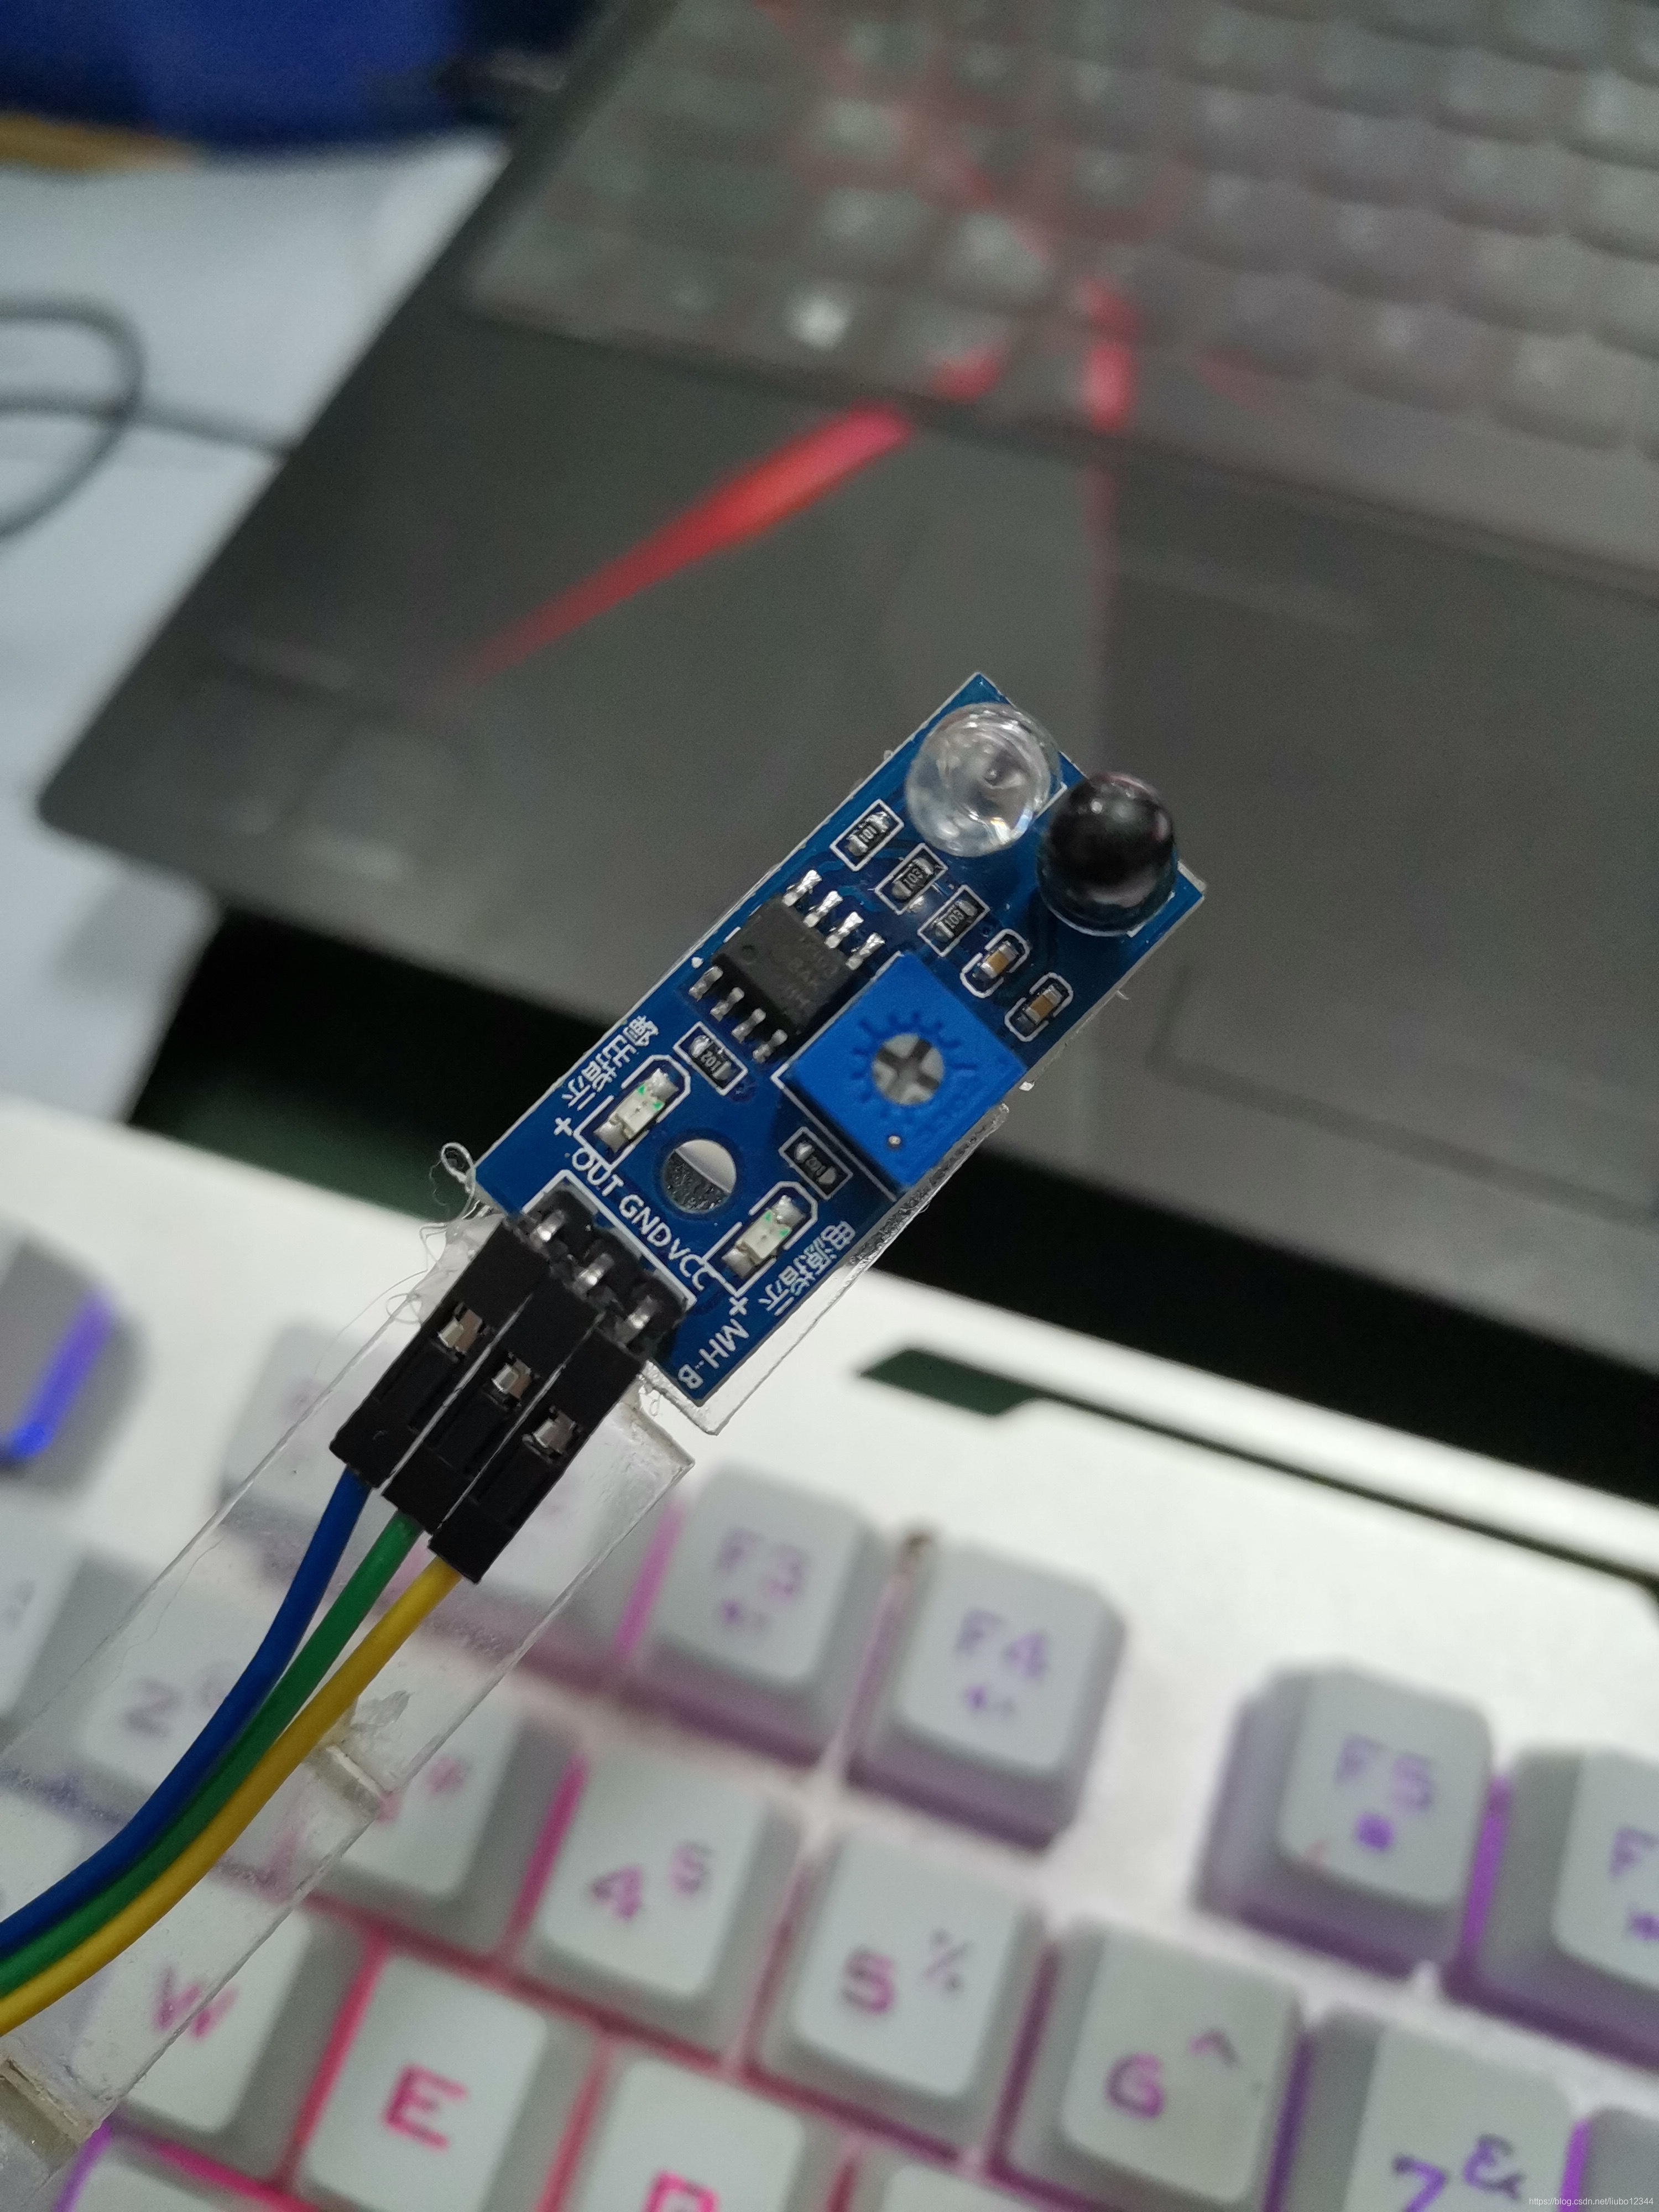
\includegraphics[width=0.5\textwidth]{figures/sensor.jpg}
  \caption{ 常见的红外传感器}
\end{figure}

常见的使用方案是在循迹车的前方布置对称的红外传感器。当线出现在红外传感器的正下方,它便会给控制电路采取行动的信号。例如当需要小车保持在黑色边线的赛道内时,如果侧边传感器有信号,则控制向另一个方向转弯。这种实现非常简单直观。

然而红外传感器的缺陷在于其只能给出是否检测到线的信息,而不能给出线的远近、角度信息,这使得它无法实现更加复杂和高效的控制算法。

\subsubsection{算法:从if-else到PID}
\label{subsec:label}
在空间上离散的点观测传感器虽然提供了有限的状态数,但这些状态足以支持基本的控制逻辑。例如,通过简单的条件判断(if-else逻辑),可以实现对小车行为的简单控制。然而,这种方法的局限性在于其缺乏灵活性,固定的控制指令可能无法在所有情况下都实现最优控制。例如,小车可能会在左右摇摆中陷入循环,导致时间和能量的浪费。

为了提高控制的精确度和灵活性,可以使用由多个点观测传感器组成的阵列,如线性CCD传感器。这种传感器阵列可以提供更丰富的信息,允许我们更细致地感知环境。以线性CCD为例,它包含多个光敏电阻,可以连续或离散地测量与特定线条之间的距离。通过将黑线居中于CCD传感器的正中间定义为基准状态,可以量化地表示出偏离这一状态的误差\cite{CCD}。

在循迹算法中引入PID(比例-积分-微分)控制算法,可以显著提高控制性能。PID控制器通过设定一个中间状态作为基准,利用传感器阵列检测到的距离作为误差输入,动态调整小车的轮速差,以保持小车在预定轨迹上的稳定运行。这种方法不仅能够实现更平滑的循迹,还能提高循迹的速度和效率。

具体来说,PID控制器的三个组成部分——比例(P)、积分(I)和微分(D)——共同作用于控制过程。比例部分响应当前误差,积分部分响应误差的累积,而微分部分则响应误差的变化率。通过调整这三个参数,可以优化小车对轨迹的跟踪性能,减少过冲和振荡,实现更稳定和精确的控制。


\subsection{更灵活高效的新方法}
\label{subsec:label}
\subsubsection{计算机视觉\cite{opencv}}
\label{subsec:label}
采用计算机视觉方法可以为系统获得更广的感受野和更复杂的信息。传统的方式是首先获取图像,把图像转化成灰度图再进行二值化,得到黑白图像。黑色点的平均横坐标反映了循迹线的倾斜程度。据此,可以设置阈值或PID使得小车保持循迹。
\begin{figure}[ht]
  \centering
   \begin{subfigure}[b]{0.3\textwidth}
     \centering
     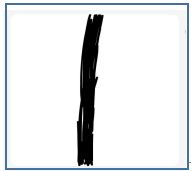
\includegraphics[width=\textwidth]{figures/straight.png}
     \caption{直行}
     \label{fig:label}
   \end{subfigure}
   \hfill
 \begin{subfigure}[b]{0.3\textwidth}
   \centering
   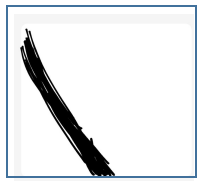
\includegraphics[width=\textwidth]{figures/left.png}
   \caption{左转}
   \label{fig:label}
 \end{subfigure}
 \hfill
 \begin{subfigure}[b]{0.3\textwidth}
   \centering
   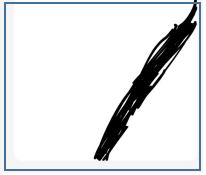
\includegraphics[width=\textwidth]{figures/right.png}
   \caption{右转}
   \label{fig:label}
 \end{subfigure}
 \hfill
  \caption{经过灰阶化-二值化的图像}
\end{figure}

在嵌入式系统的单片机应用中,矩阵运算的复杂性往往导致处理时间的增加,这直接影响了移动机器人的运行速率。为了解决这一问题,对算法进行优化显得尤为关键。优化的首要步骤是识别并筛选出对决策过程至关重要的信息。具体而言,只有那些与机器人距离较近的物体才应当被纳入考虑范围,而其他无关部分则可以被忽略,从而减少不必要的数据处理。

进一步地,图像序列中的黑色轨迹可以通过间隔采样的方式来提取,而不是对每一帧图像进行详尽的分析。这种方法可以显著降低计算量。

此外,卷积操作是一种有效的技术,它能够减少需要处理的数据量,通过识别图像中的关键特征来简化问题。通过采用池化技术,我们可以将矩阵划分为多个较小的区域,每个区域的大小与卷积核相匹配。在这些区域中,我们可以选择使用区域内元素的最大值或平均值来概括该区域的特征,从而实现对整体特征的高效替代。


\begin{figure}[ht]
  \centering
 \begin{subfigure}[b]{0.4\textwidth}
   \centering
   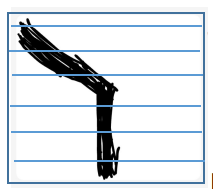
\includegraphics[width=\textwidth]{figures/jumpscan.png}
   \caption{间隔采样}
   \label{fig:label}
 \end{subfigure}
 \hfill
 \begin{subfigure}[b]{0.4\textwidth}
   \centering
   \includegraphics[width=\textwidth]{figures/pooling.png}
   \caption{最大值池化}
   \label{fig:label}
 \end{subfigure}
 \hfill

\end{figure}
\newpage
\subsubsection{强化学习}
\label{subsec:label}
2024年Yu Cao等人进行了深度强化学习循迹机器人的理论研究\cite{cao2024path}。他们将机器人与线路的横向偏差、机器人与路径之间的方向误差、机器人的速度和角速度等信息作为状态,而将机器人速度的变化率作为行动。在奖励函数中纳入与误差成正比的惩罚、与速度成正比的奖励以及惩罚机器人在困难弯道停下的参数。

\begin{figure}[ht]
  \centering
  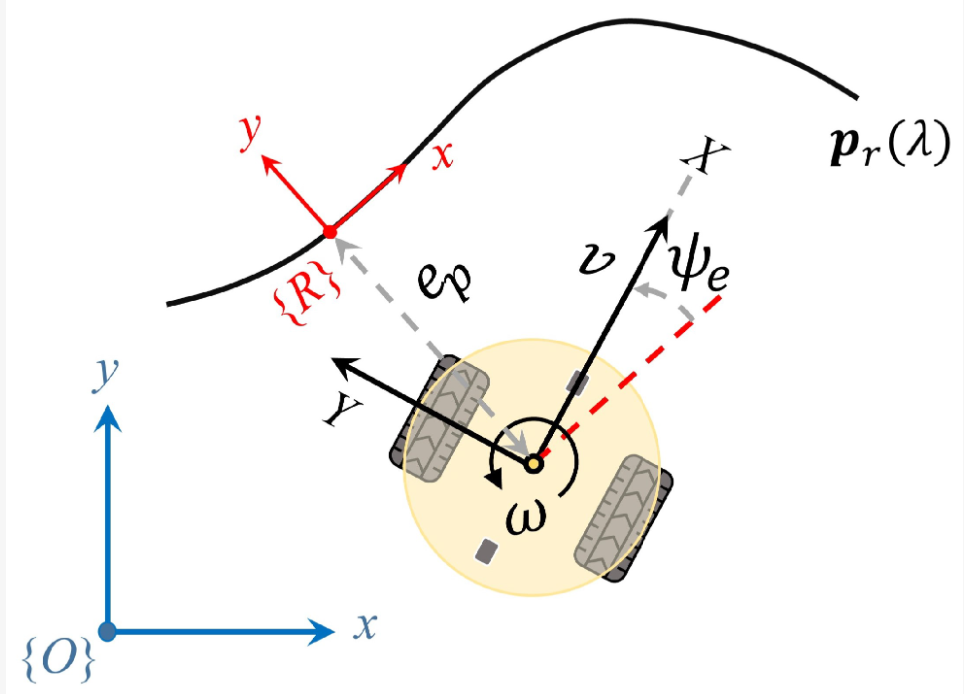
\includegraphics[width=0.5\textwidth]{figures/state.png}
  \caption{状态定义物理量\cite{cao2024path}}
\end{figure}

\[ r\left(t\right)=-k_{1}\left|e_{p}\left(t\right)\right|+k_{2}v\left(t\right)\left(1-\frac{1}{e_{tol}}\left|e_{p}\left(t\right)\right|\right)-k_{3}F\left(t\right) \]

在随机生成的环境中进行了50万次交互之后,机器人的路径实现收敛。相比传统的PP控制方法,采用深度强化学习的机器人有了自适应的速度控制能力,可以适应不同曲率的路径,还有相当不错的泛化能力,在随机生成的不同路径中均有优秀的效果。

根据现实硬件情况在Webbot中建模并进行虚拟环境的预训练,再将完成训练的模型下载到实际小车中,就可以实现该方法的实际运用。
\section{避障研究综述}
\label{sec:label}
\subsection{需要获取的信息和相关传感器}
\label{subsec:label}
\subsubsection{障碍物信息}
\label{subsec:label}
\paragraph{红外避障传感器}

红外传感器的工作原理基于一对红外发射器和接收器的配合。发射器发出特定频率的红外光波,当这些光波遇到障碍物时,它们会被反射回来并被接收器捕捉。在传感器的正前方如果存在障碍物,传感器将输出低电平信号;相对地,如果传感器的探测范围内没有障碍物,它将返回高电平信号。

红外传感器的测距机制采用的是三角测量法。这种方法的一个显著特征是,白色物体由于其较高的反射率,能够被检测到更远的距离;而黑色物体由于较低的反射率,其可探测距离相对较短。此外,红外传感器无法有效检测透明物体或接近黑体的物体。物体的面积大小也会影响其可探测距离,面积较大的物体可以被探测到更远的距离,而面积较小的物体则探测距离较短。传感器还能够检测到偏移角度达40°的物体,并且其响应速度通常优于超声波传感器。

值得注意的是,当障碍物距离传感器非常近时,反射回来的红外光波的强度(L值)会显著增加,可能超出电荷耦合器件(CCD)的探测极限。相反,当障碍物距离传感器较远时,L值会减小,这可能导致测量精度下降\cite{jh1}。这些特性对于传感器的应用场景和精度要求具有重要影响。


  \begin{figure}[ht]
    \centering
    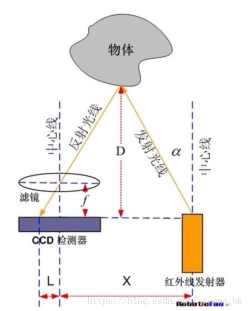
\includegraphics[width=0.5\textwidth]{figures/hongwaibizhang.png}
    \caption{红外避障原理 }
  \end{figure}
\newpage
  \paragraph{超声波传感器}
超声波传感器的核心组件包括压电晶体和镍铁铝合金两种材料。利用压电效应,压电晶体构成的传感器能够实现能量的双向转换:将电能转换为机械振动以产生超声波,同时在接收到超声波时,也能将其转换回电能。

超声波具有波长短、频率高、绕射效应小以及方向性好的特点。在传感器的操作过程中,发射器产生机械振动,发射出超声波;当超声波遇到目标物体时,会发生反射或折射,随后由接收器捕获回波并将其转换为电信号进行处理。由于超声波的传播速度是已知的,通过测量发射和接收之间的时间差,可以计算出传感器与物体之间的距离。此外,结合传感器发射器和接收器之间的距离,可以进一步确定障碍物的确切位置。

超声波传感器以其低成本、简单的实现方法和成熟的技术而著称。然而,在进行高精度测量时,必须考虑温度、湿度等环境因素对测量结果的影响。通常,超声波传感器的有效作用距离较短,其探测范围一般在米级,但存在毫米级的探测盲区。由于超声波以锥形波束传播,它能够探测到的是在特定锥形角度范围内最近物体的距离。

超声波传感器的局限性包括较长的测距时间、相对较低的感应精度,以及容易受到其他超声波传感器的干扰,这可能导致测量结果中出现较多的噪声点。
\begin{figure}[ht]
    \centering
    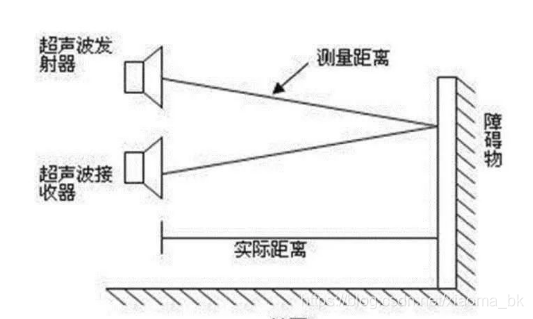
\includegraphics[width=0.5\textwidth]{figures/super.png}
    \caption{超声波测距原理 }
  \end{figure}

  \paragraph{激光雷达}
  
在润色这段关于激光雷达原理和测量方案的描述时,我会采用更加专业和精确的语言,同时确保文本的流畅性和逻辑性。以下是润色后的段落:

激光雷达的工作原理涉及发射和接收激光束,它可以通过两种主要方式进行测量:一种是利用三角测量原理,类似于红外避障;另一种是利用时间差和速度的测量,类似于超声波。激光雷达系统由发射器和接收器组成,发射器发射激光照射目标物体,而接收器则捕获返回的光波。

机械式激光雷达包含一个装有反射镜的机械结构,通过反射镜的旋转,激光束能够在一个平面上进行扫描,从而获取该平面上各个点的距离信息。

在测量方案方面,主要有两种技术路线:基于飞行时间(Time of Flight, TOF)的测量和三角测距。TOF的基本原理可以用公式 \( d = \frac{ct}{2} \) 表示,其中时间 \( t \) 的测量是整个过程中最关键的部分。时间测量的方法主要有三种:第一种是直接测量法,通过脉冲激光直接测量传播时间,但由于光速极高,这种方法对时间测量设备的精度要求极高,导致成本昂贵;第二种是差频测量法,通过发射调频连续波并测量反射波之间的频率差来确定时间;第三种是相移测量法,传感器以已知频率发射调制光,并测量发射信号与接收信号之间的相位差,从而根据调制波的波长和相位差计算出距离。

三角测距的原理与红外测距相似,此处不再详细描述。

激光雷达在测距方面具有一些显著特点:测量的可靠性与接收信号的幅度平方成反比,具有高角度分辨率和高测距精度。然而,它在测量远距离物体和黑色物体时可能存在困难,透明材料的测量也较为复杂。此外,激光雷达的成本较高,价格昂贵;采用三角测距的激光雷达在量程上通常受到限制,一般不超过几米,并且精度相对较低\cite{jh1}。

  \paragraph{毫米波雷达}
  
毫米波雷达是一种先进的雷达传感器,它利用毫米波段的电磁波来测量距离、相对速度和方向等参数。在车辆行驶过程中,毫米波雷达向前方发射电磁波脉冲。当这些脉冲遇到障碍物时,会反射回来形成回波。通过对这些反射波的频率变化进行分析——即发射频率与接收频率之间的差值——可以检测到前方或对面是否存在障碍物、障碍物的距离、相对速度以及它们的方向。

毫米波雷达的工作原理与前述雷达技术相似,但它具有一些独特的特性。首先,毫米波雷达的检测距离较长,能够覆盖更远的范围。其次,它在金属表面以及夜间、逆光、雾、雨、雪等复杂环境下都能保持良好的性能。然而,对于非金属表面,如人体或纸箱等,由于反射效果不佳,毫米波雷达的检测能力会受到限制。

鉴于毫米波雷达在非金属表面检测上的局限性,以及考虑到实际的具体需求和环境条件,本次设计不将其作为备选方案\cite{jh2}。

  \subsubsection{位置信息}
  \label{subsec:label}
为了实现精确的算法,需要收集必要的位置信息,以确定小车当前所处位置以及小车已完成的路程。位置信息可以用矢量表示,因此需要一个角度信息和一个距离信息,分别由陀螺仪和里程计两种传感器测量并提供。

\subsection{避障算法}
\label{subsec:label}
智能车辆,作为一种具备自主决策能力的自动化机器人,必须能够从其周围环境中获取信息,并基于这些信息做出决策。这使得它们能够执行全局路径规划和在局部危险情况下进行避障,以确保顺利到达目的地并完成既定任务。

全局路径规划为智能车辆提供了在已知地图环境中的最优行驶路线。这种规划确保了车辆能够以最有效的方式从起点导航至终点。与此同时,局部避障算法则赋予了智能车辆对不可预见事件的即时反应能力,这对于处理突发状况和保持车辆安全至关重要。

有效的局部避障算法必须具备快速响应、高实时性和高效率的特点,它们是智能车辆避障功能的核心。这些算法需要能够迅速识别和评估周围环境中的潜在障碍,并计算出避障路径,以避免碰撞并维持车辆的正常运行。

在接下来的讨论中,我们将详细探讨全局规划算法和局部避障算法的设计原理、实现方法以及它们在智能车辆导航中的应用。

\subsubsection{全局规划算法}
\label{subsec:label}
全局规划算法是在全局地图已知(至少是起点和终点已知)的情况下规划出的最优路径,主要目的是节省时间,提高效率。下文总结了目前的部分全局规划算法。
\paragraph{A*算法}
A*算法,首次提出于1968年,是Dijkstra算法与广度优先搜索算法(BFS)的融合之作,其核心在于利用启发式函数 \( f(n) = g(n) + h(n) \) 以加速最优路径的搜索过程。

在该算法中,\( f(n) \) 代表节点的综合优先级函数,其在节点选择过程中起到决定性作用,反映了节点的总成本。\( g(n) \) 表示从起始点到节点n的实际累积成本。而 \( h(n) \) 则是对当前节点至目标点的代价进行预估的估值函数,它基于对地形或环境特征的先验设计,提供了从当前位置n到目的地的最优路径的启发式估算。理想情况下,\( h(n) \) 的值不应超过实际成本,以确保算法能够找到成本最低的路径。


三个函数定义如下:
\begin{enumerate}
\item 	h(n)(启发式函数-代价估值函数):对于网格点(x,y),目标点($x_0$,$y_0$),启发式函数可以如此定义: \( h(n)=\sqrt{(x-x_0)^2+(y-y_0)^2} \) 这个函数值实际上是当前点到重点的欧里几得距离。
\item $g(n)$ (成本函数) :每当从起始点通过路径移动到一个新节点,$g(n)$需要累加上到达该节点的移动成本。设每一步的移动成本是w,则:$g(n_{next})=g(n_{now})+w$
  \item  $f(n)$(总成本):综合上述值,得到$f(n)$评价总成本,最终从中选取节点$f(n)=g(n)+h(n)$

  \end{enumerate}

A*算法以其高效性、灵活性和广泛的适用性而著称,然而,它也存在一些局限性。启发式函数 \( h(n) \) 的选择对A*算法的准确性至关重要,不当的选择可能会导致算法无法找到解或效率降低;算法在运行过程中需要维护开放列表和封闭列表,这将存储大量的节点信息,从而消耗大量的内存资源;在动态变化的环境中,A*算法需要不断地重新计算,这可能会影响到它的实时性能;此外,在处理大型图时,由于需要评估的节点数量庞大,A*算法可能会面临计算量大和速度缓慢的问题。

为了解决这些问题,陈鑫鹏等人提出了一种改进的算法,即等步长分层拓展算法,旨在优化A*算法的性能。该算法通过调整启发式函数和节点扩展策略,以期在保持算法高效性的同时,提高其在特定环境下的适应性和准确性。通过这种方法,可以在一定程度上缓解上述问题,提升A*算法在复杂场景下的应用效果\cite{jh3}。

\paragraph{$D^{*}$算法}
D*算法,亦称为动态A*算法,是在A*算法的基础上发展起来的,最初应用于火星探测器的路径规划。

与A*算法从起点到终点的单向正向搜索不同,D*算法采用的是反向搜索策略,即从终点到起点进行搜索。它利用先前的搜索结果,通过再利用信息实现高效的路径搜索,显著缩减了搜索范围和时间。这种方法特别适用于周围环境未知或存在动态变化的情况。D*算法在初始假设中认为地图上没有障碍,起点到终点的路径为直线,然后在在线运行时不断进行路径的重新规划,以适应全地图未知的路径规划需求。

在D*算法的研究和发展中,秦旭等人对传统D*算法进行了优化。他们改进了子节点的选择策略,并对代价估计函数进行了调整,同时引入了平滑度函数,这些改进使得规划时间减少了20\%。此外,张希闻等人提出了一种扩展Moore型元胞结构的方法,进一步缩短了原D*算法的路径。通过将传统的八点邻接结构扩展到十六点,新算法不仅提高了路径规划的速度,但也相应地增加了空间复杂度。这些改进为D*算法在动态环境中的应用提供了更多的可能性和更高的效率\cite{jh4}。
\newpage
\paragraph{遗传算法}

遗传算法(GA)是John holland 在20世纪70年代初提出的根据生物体进化规律而设计的\cite{jh5}。它是一种全局最优解搜索的启发式优化算法,机制是模拟达尔文进化理论和自然界优胜劣汰。算法流程如下:
\begin{figure}[ht]
  \centering
  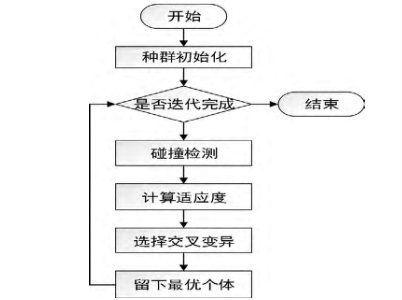
\includegraphics[width=0.5\textwidth]{figures/yichuan.png}
  \caption{遗传算法}
\end{figure}

\paragraph{蚁群算法}

由Marco Dorigo 在1992年提出,是一种用于寻找优化路径的随机搜索算法\cite{jh5}。思路是将城市与城市之间的路径看作一幅图,放置n只蚂蚁在图中移动。每只蚂蚁成功到达终点的路径上会留下信息素,信息素最大的部分就是最优路径
\begin{figure}[ht]
  \centering
  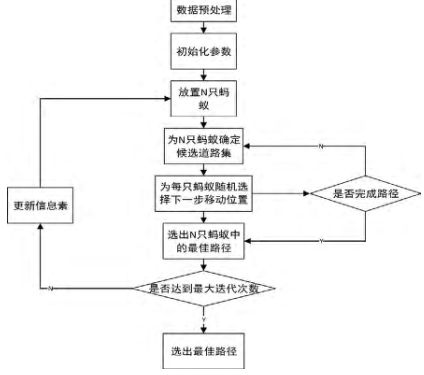
\includegraphics[width=0.5\textwidth]{figures/yiqun.png}
  \caption{蚁群算法 }
\end{figure}
\newpage
\subsubsection{局部避障算法}
\label{subsec:label}
局部避障算法属于动态规划,主要信息来源是无人车传感器提供的环境信息。此种算法的设计目的是为了让机器人能够灵活调整决策,并尽快对路径上的算法做出响应,根据特点可以分为采样方法、条件约束法和机器学习法。常用的局部路径算法包括人工势场法和虚拟力场法。
\paragraph{人工势场法\cite{jh6}}
人工势场法(Artificial Potential Field, APF)是一种基于虚拟力的路径规划方法,它将车辆在环境中的导航问题转化为在人工构建的势场中寻找路径的问题。在这种方法中,目标点被视为一个引力源,对车辆产生吸引作用,促使车辆向目标方向移动;而障碍物则被视为斥力源,对车辆产生排斥作用,以避免碰撞。车辆的运动是由这两种力的合力所决定的,通过计算合力的方向和大小,车辆能够沿着势场的下降方向移动,从而找到一条既无碰撞又相对最优的路径。

引力势场主要与汽车和目标点之间的距离有关。距离越大,汽车所受的势能值就越大;距离越小,汽车所受的势能值就越小。因此,引力势场的函数是:
$$U_{att}(q)=\frac12\eta\rho^2(q,q_g)$$

其中$\eta$是正比例增益系数,$\rho(q,q_g)$是一个矢量,标识汽车的位置$q$和目标点位置$q_g$之间的欧式距离$|q-q_g|$,矢量方向是从汽车的位置指向目标位置,相应的引力$F_att(q)=-\nabla U_{att}(q)=-\eta\rho(q,q_g)$,是引力场的负梯度,代表引力势场函数$U_att(q)$变化最快的方向。

决定障碍物斥力势场的因素是汽车与障碍物之间的距离。当汽车没有进入障碍物的影响范围时,其受到的势能为 0;汽车进入障碍物影响范围后,汽车受到的势能与距离的关系呈负相关。设车辆当前和目标点的距离为$\rho_g^n$,其中$n$自行定义。具体公式如下:
$$U_{req}(q)=\begin{cases}\dfrac{1}{2}k\left(\dfrac{1}{\rho(q,q_g)}-\dfrac{1}{\rho_0}\right)\rho_g^n,&\quad0\leq\rho(q,q_g)\leq\rho_0,\\\\0\:,&\quad\rho(q,q_g)>\rho_0\end{cases}$$
$F_{req1}$方向为障碍物指向车辆;$F_req2$方向为车辆指向目标点;$F_req$为斥力势场的负梯度作用力。即斥力势场的负梯度作用力等于障碍物指向车辆的斥力和车辆到目标点的斥力之和。
\begin{align}
  \label{}
F_{req}&=F_{req1}+F_{req1}\\
F_req1&=k\left(\frac1{\rho(q,q_g)}-\frac1{\rho_0}\right)\frac{\rho_g^n}{\rho^2(q,q_g)}\\
F_req2&=\frac n2k\left(\frac1{\rho(q,q_g)}-\frac1{\rho_0}\right)^2\rho_g^{n-1}
\end{align}
\begin{figure}[ht]
  \centering
  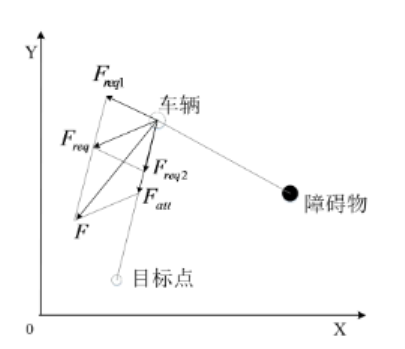
\includegraphics[width=0.5\textwidth]{figures/APF.png}
  \caption{车辆在改进后势场中的受力}
\end{figure}

根据上述定义的引力场和斥力场函数,可以得到整个空间的复合场,机器人合力势场大小为机器人所受斥力势场和引力势场之和,故合力势场总函数是:
\[ U(q)=U_{att}(q)+U_{req}(q) \]
所受合力是:
\[ F(q)=-\nabla U(q)=F_{att}(q)+F_{req}(q) \]
合力方向决定汽车的行驶朝向;合力大小决定汽车的行驶加速度。
\newpage
应用人工势场法规划出来的路径一般比较平滑安全、算法简明,实时性良好。但是算法也有一些缺点:
\begin{enumerate}
\item 当目标点附近有障碍物时,斥力远远大于引力,车辆将很难到达目的地。
\item 当智能车在某一点引力和斥力刚好大小相等时,车辆会陷入局部最优点。
\item 当车辆到达障碍物附近时,人工势场模型产生的轨迹将出现抖动,不光滑\cite{jh8}。
\item 当引力过大时,即无人车位于起始位置时,无人车可能会忽略障碍物斥力的作用造成碰撞\cite{jh7}。
  \item 传统人工势场只考虑了障碍物与目标点静止不动的静态环境,而车辆实际是在运动的环境中,因此在动态环境下无法取得良好的效果。
\end{enumerate}
针对这些问题,学界产生了很多改进措施。

在研究领域中,王会丽等人通过优化势场函数,有效地解决了局部最优解的问题,成功地识别并定位了全局最优解。李钧泽等人对引力与斥力模型进行了创新性改进,显著提升了算法在避免与原目标端障碍物碰撞以及确保目标可达性方面的性能。此外,他们引入了临时障碍物的概念,进一步优化了解决局部极小值问题的方法。余震中等人则采用了势场强度来替代传统的力矢量,通过在障碍物斥力函数中引入一个系数项,有效地解决了障碍物与目标点距离过近导致的可达性问题。在动态环境下,考虑到移动速度与机器人速度的相互影响,他们引入了速度信息,从而为移动机器人的路径规划提供了一种新的解决方案\cite{jh5}。

\paragraph{模糊逻辑算法}

模糊逻辑算法作为一种广泛应用于在线路径规划的算法,其实施流程通常遵循模型构建和局部路径规划的顺序。该算法的构建并非基于特定对象的数学建模,而是通过观察和记录驾驶员的操作行为,将人类驾驶经验转化为控制指令。在避障路径规划过程中,环境信息经过模糊化处理,并通过模糊规则的连续查询来生成规划结果。部分学者进一步发展了动态模糊环境模型,该模型利用模糊集合来表征环境中运动物体的状态,包括其位置、速度及其方向等属性。随后,通过应用模糊规则对不同方向进行综合评估,以得出最优搜索路径。

模糊算法的优势在于其对车辆的精确定位要求不高,因而展现出较强的鲁棒性,能够适应各种未知环境,并提供有效的路径规划。然而,模糊算法的局限性在于其缺乏自学习能力,一旦模糊规则被设定,便难以根据新的情况进行调整,这限制了算法的灵活性和适应性\cite{jh6}。

\chapter{原型设计方案}

\section{机械设计}
\subsection{车体}
\label{subsec:label}
针对车体的驱动机构设计,我们计划采用一种创新的结构配置,即两个前轮驱动轮结合一个后轮万向轮,形成一种近似倒三角型的车体构型。在车体的纵向布局上,我们采用了双层结构设计,其中下层专门用于安装电机、电池、机械夹爪以及舵机等关键组件。而上层则专门配置了控制硬件和通信硬件,包括但不限于STM32微控制器、电压转换模块、蓝牙通信模块以及超声波传感器等。为了提升OpenMV摄像头的工作效能,我们将其置于一个较高的位置,以扩大其观测范围,从而提高环境感知能力。
\begin{figure}[ht]
  \centering
  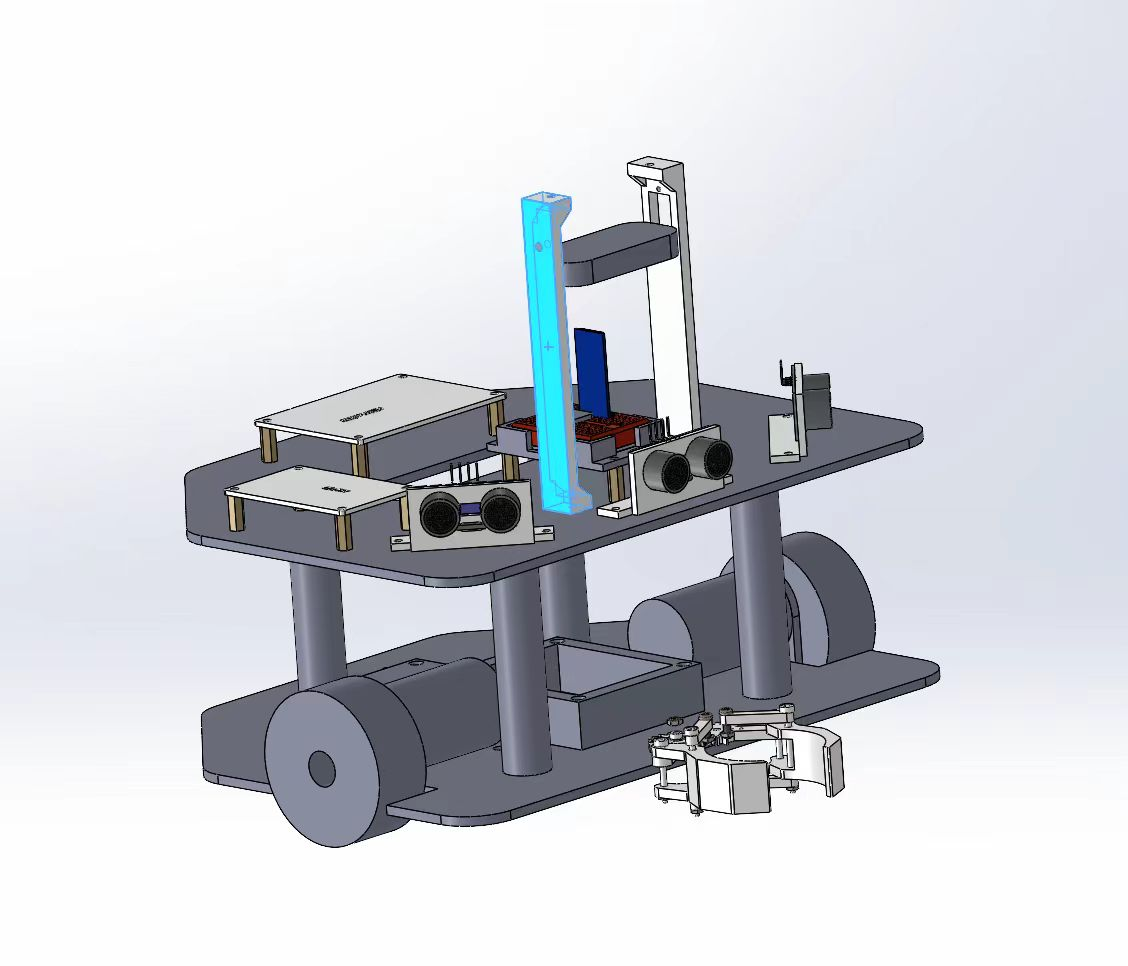
\includegraphics[width=0.5\textwidth]{figures/body.jpg}
  \caption{车体原型}
\end{figure}
\newpage
\subsection{抓取机构}
在设计抓取机构时,我们必须确保其既能满足摩擦力的要求以稳定夹取物体,同时又要避免过大的尺寸,以防遮挡传感器并干扰其正常运作。经过综合评估机械夹爪、吸盘和仿生结构的优缺点,我们最终选择了一种单自由度的机械夹爪结构。该结构利用电机的旋转驱动齿轮,进而使机械夹爪实现转动,实现一个电机同时控制两侧夹爪的同步运动。夹爪的上下两端各配备一对连杆,用以固定和限位,并通过螺栓和螺母等紧固件进行加固,以确保夹取机构的稳定性和可靠性。

为了防止在抓取货物后,由于颠簸或碰撞导致货物底部与赛道表面摩擦,可能引发的货物滑落或对小车运动的干扰,我们设计了一种机制,使得夹取机构在抓取货物后能够向上翻转,将货物抬升,从而避免这些问题的发生。同时,我们确保抬升后的货物不会对传感器造成干扰,以维持传感器的正常工作状态。
\begin{figure}[ht]
  \centering
  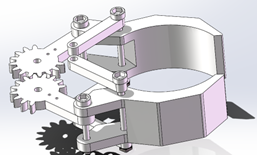
\includegraphics[width=0.5\textwidth]{figures/pickup.png}
  \caption{抓取机构概念图 }
\end{figure}
\newpage
\section{测量}
\label{sec:label}
\subsection{小车位姿测量}
\label{subsec:label}
为了对小车进行定位以及进行下一步的计算,我们需要对小车的位姿进行测量。综合考虑各种传感器的性能之后,我们初步决定采用里程计的方式测量小车移动的距离,用陀螺仪测量小车转过的角度,从而确定小车的位姿。
\subsection{循迹中的测量}
\label{subsec:label}
由于我们计划采用视觉循迹方案,所以需要实时图像等视觉数据。我们计划采用OpenMV视觉传感器,其具备计算处理能力,有利于提高图像处理帧率,同时封装性良好,便于我们在短时间内快速学习并应用。
\subsection{避障中的测量}
\label{subsec:label}
我们计划采用激光测距传感器获取距离信息为主,辅以OpenMV视觉传感器进行目标识别。如此可以充分利用OpenMV获得的二维图像信息与较好的前瞻性,并用激光测距测量小车其他方向距障碍物的距离作为补充,并且通过随机算法与人工势场法的加权实现小车前进方向的实时更新,之后会在实现中具体论证可行性。
\section{循迹}
\label{sec:label}

在进行路径追踪方案的选择时,我们经过综合考量,决定采用视觉循迹技术。在文献综述中,我们考察了四种主要的循迹方案:点传感器(包括红外传感器和光敏电阻)、线性CCD、视觉循迹以及强化学习循迹。点传感器方案由于其离散的状态限制,导致控制算法的设计空间受限,且在循迹的平滑性和速度方面未能达到理想的效果。线性CCD虽然可视为点传感器的扩展,但其信息获取的精度和前瞻性仍然有限。

强化学习循迹方案虽然具有较高的灵活性和适应性,但其实现需要复杂的环境感知能力,并且必须在虚拟环境中进行大量的预训练以获得收敛的路径。考虑到实现难度较大,以及我们现有的硬件资源——特别是笔记本电脑显卡的算力限制,我们决定不将其作为首选方案。
\subsection{视觉传感器选择}
\label{subsec:label}
在视觉传感器的选择上,我们决定采用OpenMV作为我们系统的核心组件。OpenMV的显著优势在于其集成了单片机功能,具备强大的计算处理能力,这不仅有助于提升图像处理的帧率,还能显著增强小车的整体性能。此外,OpenMV的配套开发工具具有优良的封装性,其官方文档详尽且易于理解,同时拥有丰富的开放资源。这些特性对于开发者来说,无疑能够大幅度降低学习成本,提高开发效率。
\subsection{算法选择}
\label{subsec:label}
总体上,我们的算法流程首先涉及图像的预处理阶段,随后引入PID控制策略以实现精确的路径跟踪。

我们首先利用OpenMV内置的二值化工具,对裁剪后的图像进行处理,将其转换为黑白图像,以简化后续处理步骤。接下来,我们选择视场中间靠前的区域作为感兴趣区域(Region of Interest, ROI),通过裁剪或矩阵池化技术减小数据矩阵的规模。然后,运用OpenMV自带的拟合函数对黑线进行曲线拟合,从而计算出黑线的方程。根据黑线的斜率,我们确定转向控制量,该控制量的生成将通过PID控制器进行调节,以确保转向过程的稳定性和平滑性。

值得注意的是,PID控制器的误差输入为黑线斜率与预设基准斜率之间的差值,而控制输出则体现为两轮之间的转速差,这直接影响小车的转向行为。
\section{避障算法设计}
\label{sec:label}
\subsection{避障信息获取}
\label{subsec:label}
\subsubsection{位置信息}
\label{subsec:label}
在避障过程中,为了精确确定小车的位置和方向,必须生成其矢量路径。矢量路径包含两个关键信息要素:角度和距离。角度信息的获取依赖于陀螺仪,该设备能够记录小车相对于初始方位的当前方位角度。而距离信息的获取则通过里程计模块实现。

具体而言,我们使用陀螺仪来监测小车当前方位与初始方位之间的夹角变化。当监测到的角度变化在任意一侧超过90度,并且小车行走的距离超过了当前总行程的一定比例时,我们将执行停止前进并原路返回的操作。

对于距离的测量,我们采用里程计模块,具体通过编码器来记录主动轮的转动圈数。随后,利用一系列数学公式将编码器记录的圈数转换为小车在当前方向上实际行走的距离,并进行相应的记录。
\subsubsection{障碍物信息}
\label{subsec:label}
避障需要找到障碍物的位置。我们预计是使用超声波雷达获得与障碍物的距离信息。我们预计采用人工势场法,因此只需要识别前方已有的障碍物并给出当前距离即可收集障碍物信息。
\subsection{避障算法设计}
\label{subsec:label}
避障预期采用人工势场法。依据文献调研结果,结合小车所处的环境状况,预计对人工势场法作出以下改进:
\subsubsection{数学模型改进}
\label{subsec:label}
根据文献调研,人工势场法在使用过程中会出现一些问题,如因障碍物和终点距离太近导致已经到达势能零点、出现局部最优点等。针对这些问题,将数学模型更新如下。

根据梅艺林等人在2024年的工作\cite{jh7},引力势场的数学模型可以更新成如下形式:
\[ U_{att}(q)=k\frac1{\left(1+e^{\delta\Delta\rho(q,q_g)}\right)^2}+\alpha\Delta\rho(q,q_g) \]

对其求负梯度,改进引力场计算公式:

\[ F_{att}(q)=-\omega\frac{e^{\delta\Delta\rho(q,q_g)}}{\left(1+e^{\delta\Delta\rho(q,q_g)}\right)^2}+\alpha  \]
其中$\omega$引力增益系数,$\delta$是引力变化范围调节因子,$\alpha$是引力上下限调节因子。

改进的斥力势场公式如下:
\[ U_{req}(q)=k\Delta\rho(q,q_g)-k\frac{\ln{(e^{\eta\Delta\rho(q,q_g)}+1)}}{\eta} \]
对其求负梯度,改进斥力场计算公式:
\[ F_{req}(q)=k\frac1{1+e^{\eta\Delta\rho(q,q_g)}} \]
其中k是斥力大小系数,$\eta$是斥力作用范围调节因子,$\Delta\rho(q,q_{g})$是与$\rho(q,q_{g})$相关的调节因子
\subsubsection{思路改进}
\label{subsec:label}
首先,将终点所在直线设定为一级引力场,促使小车不断向最远端行进,以此避免小车可能出现的折返问题;当到达一级引力场时,旋转小车角度与引力场直线方向一致,并向前行进,如果摄像头在地面上识别到终点圆圈,进行放置的步骤;如果摄像头到达墙后仍没有终点圆圈,旋转180度,回到一级引力场,重新向前遍历。

\section{数据通信和回传}
\label{sec:label}
\subsection{蓝牙模块}
\label{subsec:label}
针对我们的场景,考虑到通信距离较短且需要具备一定的抗干扰性能,我们选择了蓝牙模块来实现通信。蓝牙模块以其小巧的体积、易于集成的特性以及低功耗的优势,在板载设计中表现出极高的友好性。特别是蓝牙通信协议中采用的跳频-扩频机制,为我们提供了出色的抗干扰能力。2.4GHz的电磁波能够有效穿透大多数材料的障碍物,确保小车在行驶过程中能够与控制终端保持稳定的信息交换。

在众多蓝牙模块中,我们预计采用HC-05模块。HC-05模块拥有丰富的相关资料和配套的开发工具,使得学习和使用过程变得十分便捷。此外,HC-05模块具备全双工通信能力,能够实现稳定可靠的信息互传。我们将通过电脑或手机向HC-05模块发送指令,并通过该模块控制单片机,同时接收来自传感器的反馈信息。
\begin{figure}[ht]
  \centering
  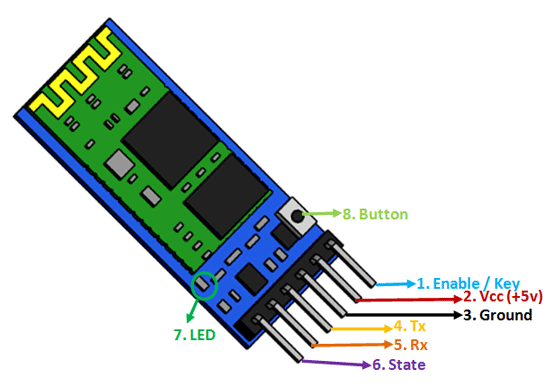
\includegraphics[width=0.5\textwidth]{figures/hc-05.png}
  \caption{\label{fig:label} }
\end{figure}
\newpage
\subsection{控制终端}
\label{subsec:label}
为了提高控制和调试的便捷性,我们计划利用蓝牙传输技术将关键数据回传至PC端,以便进行实时观察和控制。通过编码器收集的数据,我们可以准确掌握车轮的累计里程数;而陀螺仪则能够提供小车转动的角度信息。这些数据对于监控小车的运动状态至关重要。

此外,蓝牙模块还允许我们在PC终端对小车进行远程控制,包括但不限于紧急停车和转向操作。这种控制方式在小车遇到问题时尤为有用,因为它使我们能够迅速识别问题所在模块,并进行针对性的调整和调试。这不仅提高了调试的效率,也有助于快速定位并解决问题,确保小车系统的稳定运行和性能优化。
\begin{figure}[ht]
  \centering
  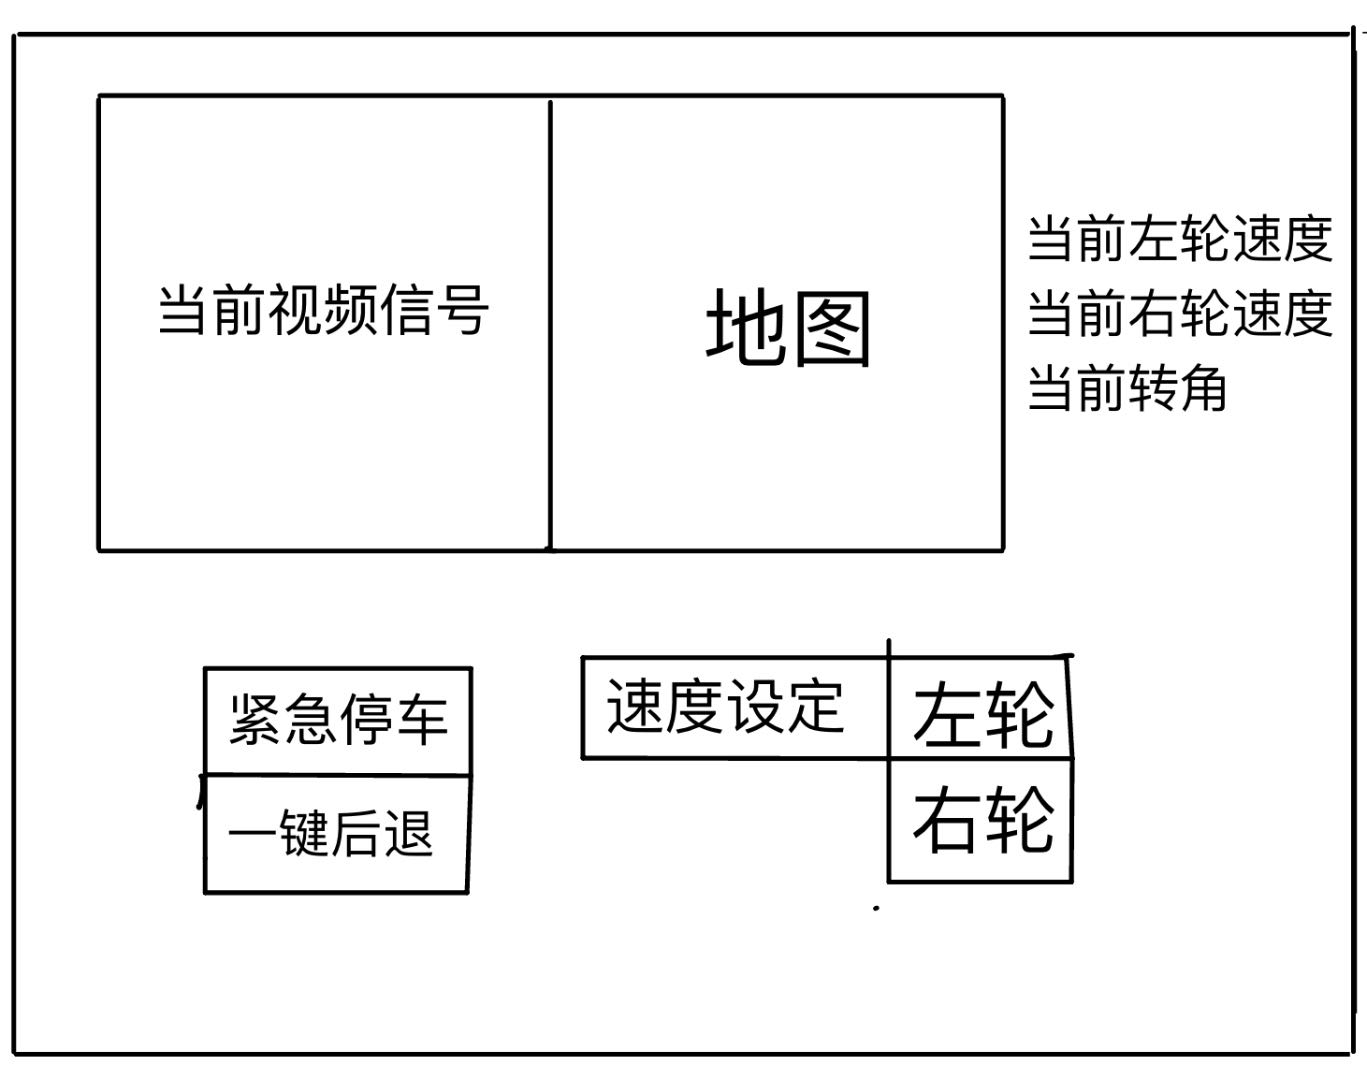
\includegraphics[width=0.5\textwidth]{figures/ui.jpg}
  \caption{控制终端UI概念图 }
\end{figure}


\section{驱动}
\label{sec:label}
\subsection{处理器}
在硬件选择过程中,我们必须综合考虑设计需求与实际的运算能力。FPGA以其出色的并发处理速度和高可靠性而著称,然而,其调试过程相对复杂。相比之下,传统的硬件解决方案可能会带来更高的技术难度。在这种情况下,采用CPU作为处理单元会相对简便。

对于我们项目中至关重要的图像处理环节,现有的STM32微控制器已经具备了足够的数据处理能力,能够满足算法的需求。鉴于我们团队成员在使用树莓派单片机方面的经验不足,同时考虑到本课程的任务进度要求,我们决定不采用树莓派单片机。相反,我们选择使用OpenMV来处理图像数据,以补充STM32的处理能力。

综上所述,我们初步计划采用以STM32为主控制器、OpenMV为辅助处理器的硬件组合方案,以确保系统的高效运行和快速开发。
\label{subsec:label}
\subsection{电机驱动}
\label{subsec:label}
选择使用PWM方法驱动,并用编码器回传电机数据。选择L298模块同时驱动两轮电机,并使用PID实现电机实际速度的准确、稳定控制。
\subsection{传感器}
\label{subsec:label}
\begin{enumerate}
\item OpenMV:自带单片机,不需要额外的驱动元件。
\item 超声波传感器:可以使用UART串口通信。
\item 里程计:里程计实际上是一个主动轮电机上的编码器,因此不需要进一步的驱动元件。
  \item 陀螺仪:不需要额外的驱动元件,使用$I^{2}C$通信。

  \end{enumerate}
  \newpage
\section{硬件清单}
\label{sec:label}
% Please add the following required packages to your document preamble:
% \usepackage{multirow}
% \usepackage{graphicx}
% \usepackage[table,xcdraw]{xcolor}
% Beamer presentation requires \usepackage{colortbl} instead of \usepackage[table,xcdraw]{xcolor}
% Please add the following required packages to your document preamble:
% \usepackage{multirow}
% \usepackage{graphicx}
% \usepackage[table,xcdraw]{xcolor}
% Beamer presentation requires \usepackage{colortbl} instead of \usepackage[table,xcdraw]{xcolor}
\begin{table}[ht]
\centering
\resizebox{0.5\textwidth}{!}{%
\begin{tabular}{|
>{\columncolor[HTML]{FFFFFF}}c |
>{\columncolor[HTML]{FFFFFF}}c |
>{\columncolor[HTML]{FFFFFF}}c |}
\hline
\textbf{类别}                                   & \textbf{名称/型号}   & \textbf{数量} \\ \hline
处理器                                           & CPU/STM32f407ZGT & 1           \\ \hline
\cellcolor[HTML]{FFFFFF}                      & OpenMV           & 1           \\ \cline{2-3} 
\cellcolor[HTML]{FFFFFF}                      & 超声波雷达           & 3           \\ \cline{2-3} 
\cellcolor[HTML]{FFFFFF}                      & IMU      & 1           \\ \cline{2-3} 
\multirow{-4}{*}{\cellcolor[HTML]{FFFFFF}传感器} & 里程计(用编码器实现)             & 1           \\ \hline
通信                                            & 蓝牙模块/HC-05       & 1           \\ \hline
\cellcolor[HTML]{FFFFFF}                      & 电机 (含直流电机和舵机)           & 3           \\ \cline{2-3} 
\cellcolor[HTML]{FFFFFF}                      & 电机驱动器/L298         & 2           \\ \cline{2-3} 
\multirow{-3}{*}{\cellcolor[HTML]{FFFFFF}动力}  & 电机上编码器              & 3           \\ \hline
\cellcolor[HTML]{FFFFFF}                      & 主动轮              & 2           \\ \cline{2-3} 
\multirow{-2}{*}{\cellcolor[HTML]{FFFFFF}车轮}  & 万向轮              & 1           \\ \hline
\end{tabular}%
}
\caption{}
\label{tab:my-table}
\end{table}
\chapter{人员分工与进度控制}
\section{人员分工}
\label{sec:label}
% Please add the following required packages to your document preamble:
% \usepackage{booktabs}
% \usepackage{graphicx}
% Please add the following required packages to your document preamble:
% \usepackage{booktabs}
% \usepackage{graphicx}
% Please add the following required packages to your document preamble:
% \usepackage{multirow}
% \usepackage{graphicx}
% Please add the following required packages to your document preamble:
% Please add the following required packages to your document preamble:
% \usepackage{multirow}
% \usepackage{graphicx}
\begin{table}[ht]
\centering
\resizebox{0.8\textwidth}{!}{%
\begin{tabular}{|c|c|c|}
\hline
姓名                   & 主要负责内容 & 辅助内容                                                                           \\ \hline
\multirow{2}{*}{邱璟祎} &硬件驱动和通讯   & \multirow{2}{*}{\begin{tabular}[c]{@{}c@{}} 识别算法\\软件\end{tabular}} \\ \cline{2-2}
                     & 循迹算法   &                                                                                \\ \hline
\multirow{3}{*}{周俊豪} & 避障算法   & \multirow{3}{*}{\begin{tabular}[c]{@{}c@{}}硬件驱动\end{tabular}} \\ \cline{2-2}
                     & 车体设计   &                                                                                \\ \cline{2-2}
                     & 运动控制   &                                                                                \\ \hline
\multirow{2}{*}{张峻瑜} & 机械臂设计   & \multirow{2}{*}{\begin{tabular}[c]{@{}c@{}}车体建模\\硬件驱动\end{tabular}} \\ \cline{2-2}
                     & 识别算法和软件   &                                                                                \\ \hline
\end{tabular}%
}
\caption{人员分工表}
\label{tab:my-table}
\end{table}
\newpage
\section{进度控制}
\label{sec:label}
% Please add the following required packages to your document preamble:
% \usepackage{booktabs}
% \usepackage{graphicx}
% Please add the following required packages to your document preamble:
% \usepackage{booktabs}
% \usepackage{graphicx}
% Please add the following required packages to your document preamble:
% \usepackage{booktabs}
% \usepackage{graphicx}
% Please add the following required packages to your document preamble:
% \usepackage{booktabs}
% \usepackage{graphicx}
\begin{table}[ht]
\centering
\resizebox{\textwidth}{!}{%
\begin{tabular}{@{}cc@{}}
\toprule
时间节点        & 阶段任务                        \\ \midrule
7月9日-7月11日  & 进一步完善详细设计方案,采购零件,编写部分硬件单元代码 \\
7月11日-7月15日 & 加工零部件,组装小车硬件,编写部分硬件单元代码     \\
7月15日-7月17日 & 单元控制代码编写,完成硬件测试             \\
7月17日-7月22日 & 完成单元控制代码编写和单元测试             \\
7月22日-7月24日 & 软件集成,硬件通讯部分代码编写与调试          \\
7月24日-7月25日 & 自动抓取货物与放置货物集成调试与细节优化        \\
7月26日-7月27日 & 循迹模式小车运动集成调试与细节优化           \\
7月27日-7月28日 & 避障模式小车运动集成调试与细节优化           \\
7月28日-7月29日 & 小车整体最终调试,准备比赛               \\ \bottomrule
\end{tabular}%
}
\caption{进度控制表}
\label{tab:my-table}
\end{table}
\bibliographystyle{IEEEtran}
\bibliography{references}

\end{document}

%%% Local Variables:
%%% mode: LaTeX
%%% TeX-master: t
%%% End:
